\documentclass[aspectratio=43, dvipsnames]{beamer}
\usepackage[version=4]{mhchem}
\usepackage[aboveskip=1pt, belowskip=1pt]{caption}
\usepackage{amsmath}
\usepackage{siunitx}
\usepackage{emoji}
\usepackage{pgfplots}
\pgfplotsset{compat=1.18,}

% Command to display isotopes
\newcommand{\iso}[2]{\ce{^{#1}#2}}
% Command to write overlap
\newcommand{\overlap}[2]{\left\langle#1\middle\vert#2\right\rangle}
% Command to write Rs
\newcommand{\rs}{$\text{R}_{\text{S}}$ }
% Command to draw enumitems outside the environment
\newcommand{\enumitem}[1]{%
\setcounter{enumi}{#1}\usebeamertemplate{enumerate item}% 
}
\newcommand{\boxitem}[1]{\raisebox{0.15em}{\enumitem{#1}}}
% Set caption package options
\captionsetup{labelformat=empty}

\title[SO splitting in 20O]{\texorpdfstring{$\nu0\textnormal{p}_{1/2} - \nu0\textnormal{p}_{3/2}$}{n0p1/2 - n0p3/2} spin-orbit splitting in \iso{20}{O}}

\date[EuNPC 2025]{EuNPC 2025 - Caen}

\author[M. Lozano et al.]{M. Lozano-González, B. Fernández-Domínguez, J. Lois-Fuentes \texorpdfstring{\newline}{}T. Roger, F. Delaunay}

\institute{USC-IGFAE, GANIL and LPC-Caen}

\usetheme{igfae}

\begin{document}

\maketitle

\section{Motivation}
\begin{frame}[t]{A recap on the SO splitting}
    Introduced by M. Goeppert-Mayer, the SO potential successfully reproduces magic numbers in stable nuclei.

    \begin{columns}[c]
        \begin{column}{0.55\linewidth}
            \begin{figure}
                \centering
                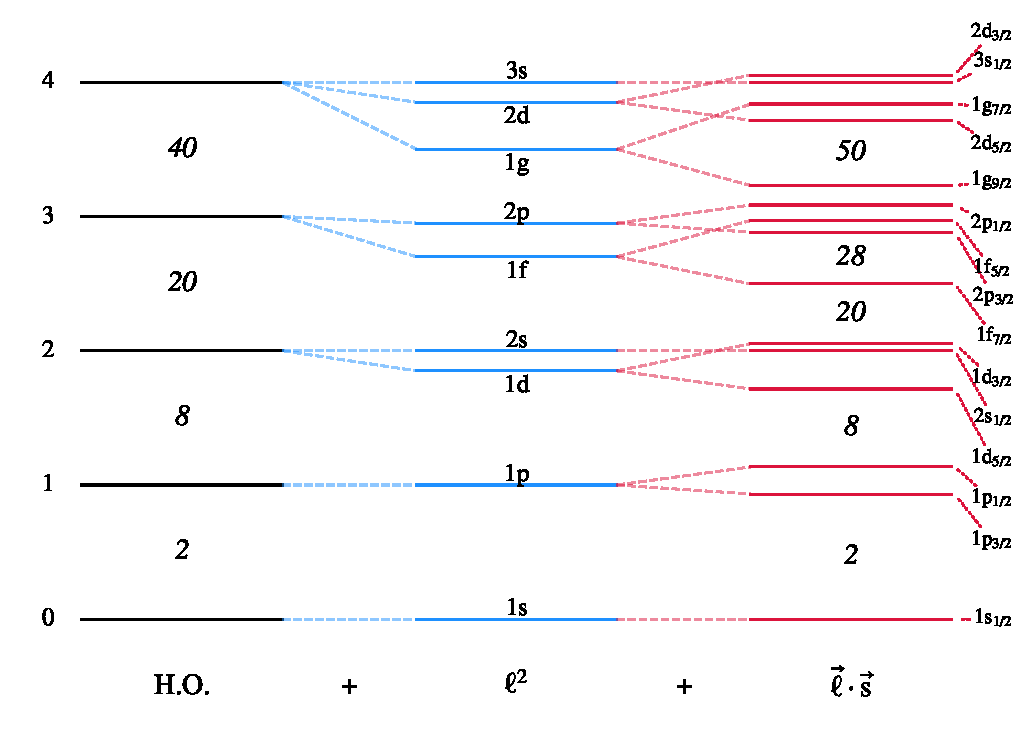
\includegraphics[width=1\linewidth]{figures/shell_model.pdf}
            \end{figure}
        \end{column}%
        \begin{column}{0.45\linewidth}
            It is mainly a surface effect:
            \begin{equation*}
                \text{V}_{\text{SO}} = - \frac{1}{\hbar^2}\text{V}_{\text{so}}(\vec{l}\cdot\vec{s})\left(\frac{1}{r}\frac{dV}{dr}\right)
            \end{equation*}
            yielding a $\ell$-dependent gap:
            \begin{equation*}
                \Delta_{\text{so}} = \frac{\hbar^2}{2}(2\ell + 1)\xi
            \end{equation*}
        \end{column}
    \end{columns}
    \mycolorbox[]{box2}{
        $\Rightarrow$ Expected to evolve towards more exotic nuclei, as surface blurs and hence $\xi \sim dV/dr$ changes.
    }
\end{frame}

\begin{frame}[t]{A recap on the SO splitting}
    G. Mairle \textit{et al.} ({\scriptsize PLB 304 (1993)}) found systematic trends easily parametrizable.

    \begin{columns}[c]
        \begin{column}{0.5\linewidth}
            \begin{figure}
                \centering
                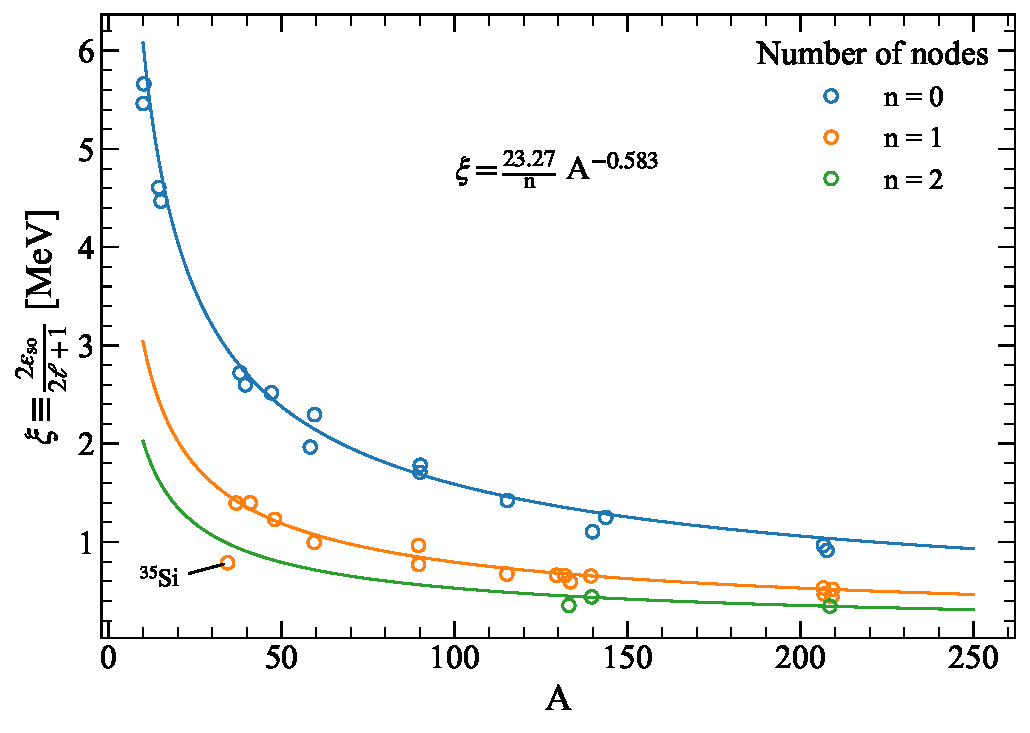
\includegraphics[width=1\linewidth]{figures/mairle_so.pdf}
            \end{figure}
        \end{column}%
        \begin{column}{0.5\linewidth}
            Deviations from the trend are found though:
            \begin{enumerate}
                \item Loosely bound orbitals
                \item Nuclear matter deplection (\iso{35}{Si}?)
                \item Role of \textbf{tensor force}
            \end{enumerate}
        \end{column}
    \end{columns}

    \begin{columns}[t]
        \begin{column}{0.5\linewidth}
            \mycolorbox{box1}{
                Proton-neutron interactions drive \textbf{shell evolution}
            }
        \end{column}%
        \begin{column}{0.5\linewidth}
            \centering
            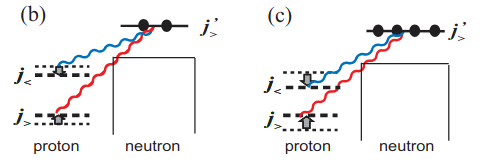
\includegraphics[width=0.9\linewidth]{figures/tensor_preliminary.png}
        \end{column}
    \end{columns}
\end{frame}

\begin{frame}{SO gap for $Z = 8$ isotopes}
    Evolution of the SO gap is plotted below for neutron-rich O isotopes.
    \begin{figure}
        \centering
        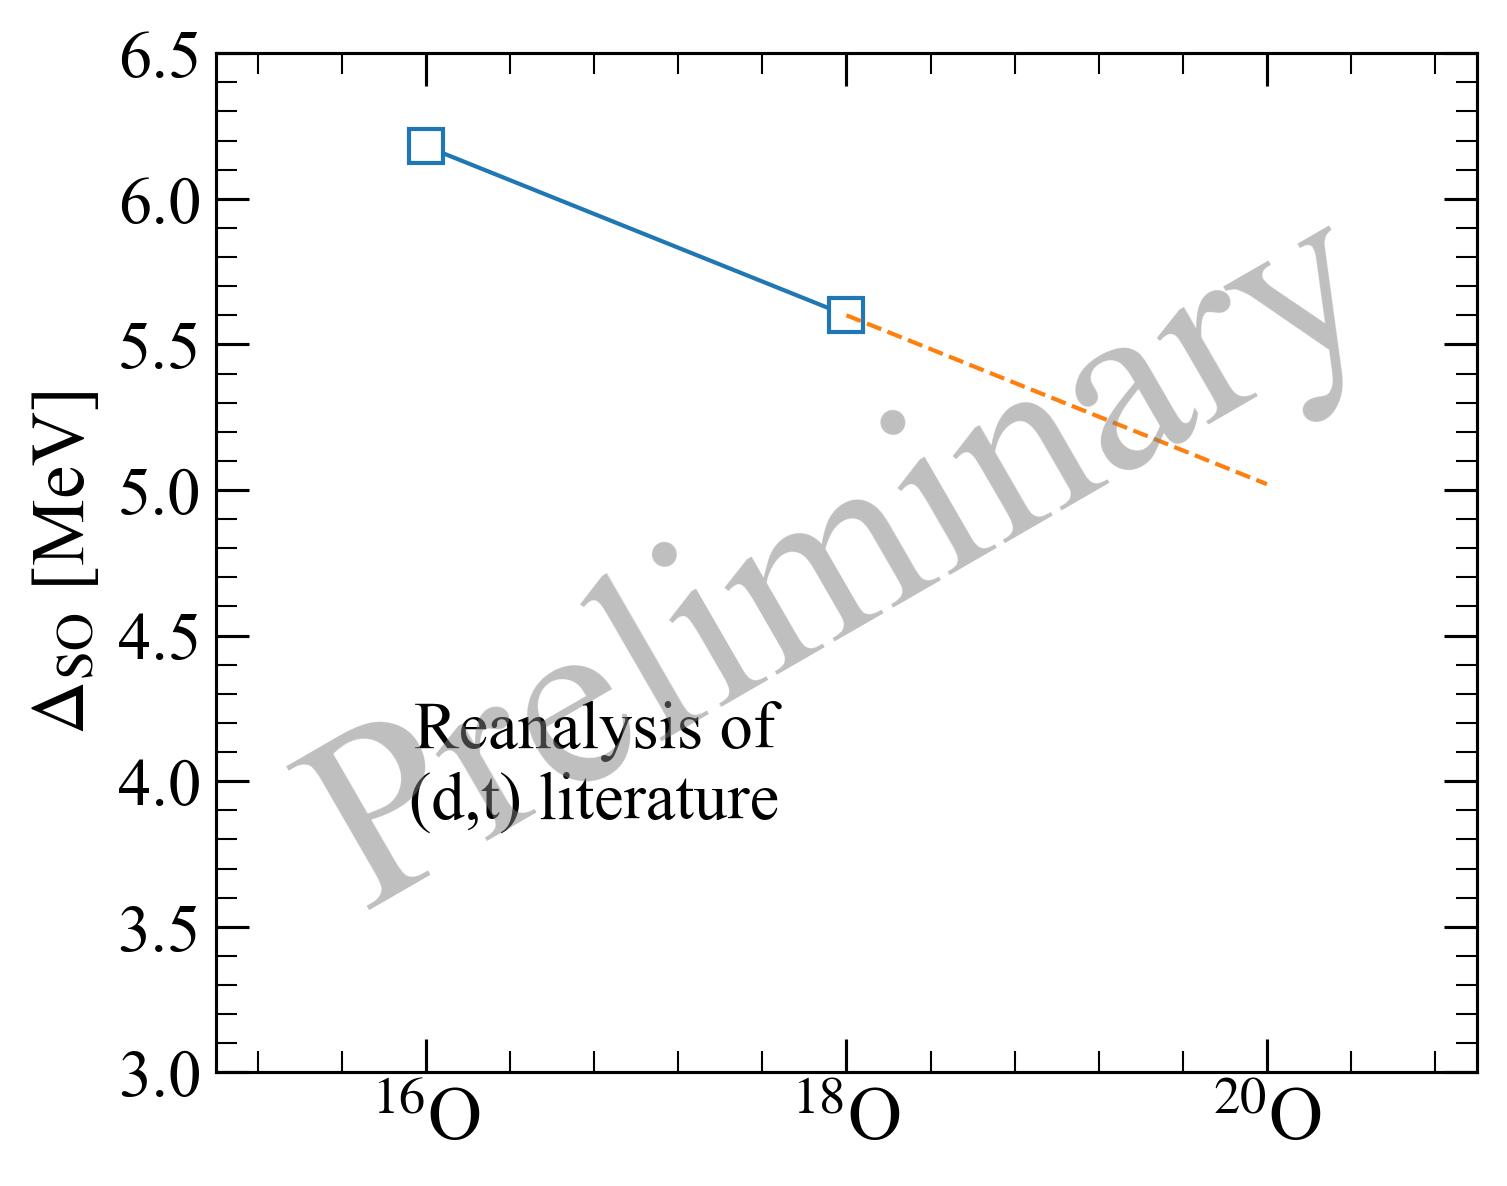
\includegraphics[width=0.5\linewidth]{figures/z6_systematics_toy.png}
    \end{figure}
    \begin{columns}[c]
        \begin{column}{0.5\linewidth}
            \mycolorbox{box1}{
                Will \iso{20}{O} follow the trend?
            }
        \end{column}%
        \begin{column}{0.5\linewidth}
            \mycolorbox{box2}{
                Could be determine tensor $\pi\nu$ contribution?
            }
        \end{column}
    \end{columns}
\end{frame}

\section{Methodology}
\begin{frame}{Experimental setup}
    E796 @ LISE in 2022. First transfer experiment with ACTAR TPC!

    \begin{figure}
        \hspace*{-0.25cm}
        % \centering
        \begin{tikzpicture}
            \node (main) at (0,0) {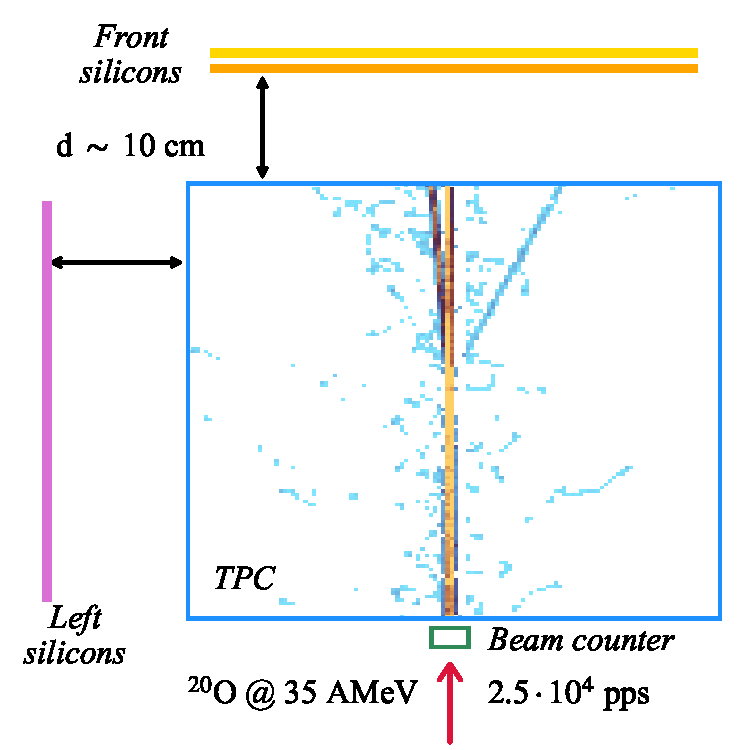
\includegraphics[width=0.5\linewidth]{figures/mini_setup.pdf}};

            % Silicons
            \node (sil) at (-4, 1.) {
                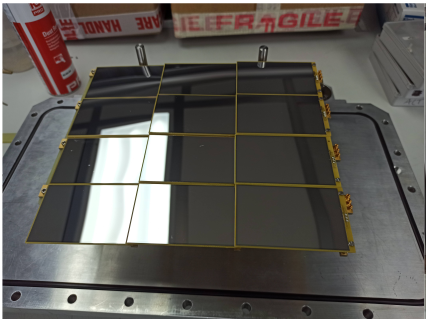
\includegraphics[width=0.25\linewidth]{figures/silicons_tese.png}
            };
            \node (siltext) at (-4.1, -1){
                \mycolorbox[0.25]{box2}{
                    \small
                    Silicon sizes:
                    $\num{80} \times \num{50} \times \num{0.5}\unit{\mm\cubed}$
                }
            };

            % TPC
            \node (tpc) at (4, 1.25){
                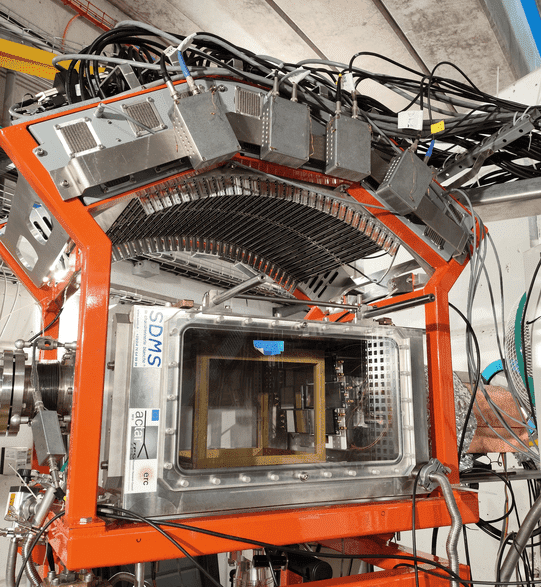
\includegraphics[width=0.25\linewidth]{figures/actar.png}
            };
            \node (tpctext) at (4.1, -1.5){
            \mycolorbox[0.25]{box3}{
            \small
            Gas setup:\\
            \qty{90}{\percent} \ce{D_2} + \qty{10}{\percent} \ce{iC_{4}H_{10}}\\
            @ \qty{950}{\milli bar}
            }
            };

        \end{tikzpicture}
    \end{figure}

\end{frame}

\begin{frame}{A window to the analysis}
    \textbf{Intricate} analysis to extract reactions of interest out of noisy data.
    \begin{columns}[c]
        \begin{column}{0.5\linewidth}
            \vspace*{-0.25cm}
            \begin{figure}
                \centering
                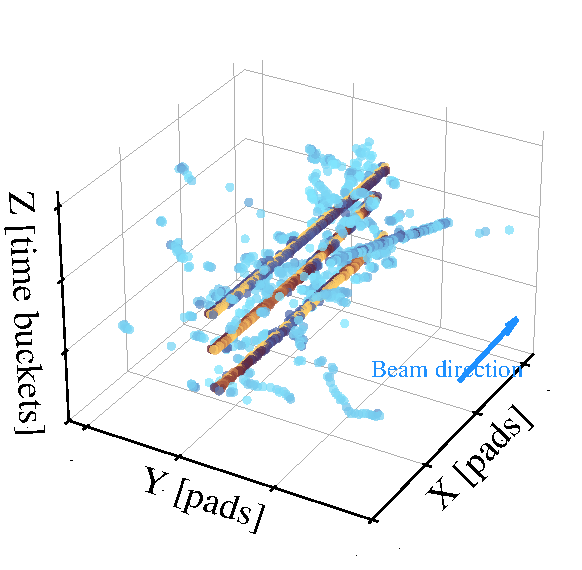
\includegraphics[width=0.8\linewidth]{figures/pure_3d.pdf}
            \end{figure}
        \end{column}%
        \begin{column}{0.5\linewidth}
            \begin{figure}
                \centering
                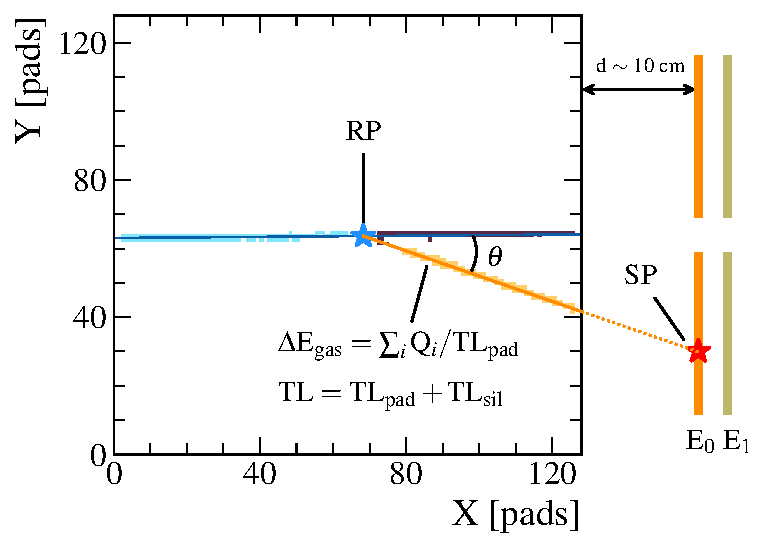
\includegraphics[width=0.95\linewidth]{figures/analysis.pdf}
            \end{figure}
        \end{column}
    \end{columns}
    Conversely, the TPC offers unique advantadges:
    \begin{columns}[c]
        \begin{column}{0.5\linewidth}
            \mycolorbox[1]{box2}{
                \boxitem{1} Precise \textbf{vertex} determination\\
                \boxitem{2} Improved $\Delta E$ corrections
            }
        \end{column}%
        \begin{column}{0.5\linewidth}
            \mycolorbox[1]{box4}{
                \boxitem{3} Factor 10 in target number\\
                \boxitem{4} Implicit PID with $\Delta E_{\text{gas}}$
            }
        \end{column}
    \end{columns}
    
    
    
\end{frame}

\begin{frame}{A window to the analysis}
    Two steps needed after data has been processed.
    \begin{columns}[c]
        \begin{column}{0.5\linewidth}
            \mycolorbox[1]{box2}{
                \boxitem{1} Triton identification in PID
                \begin{figure}
                    \centering
                    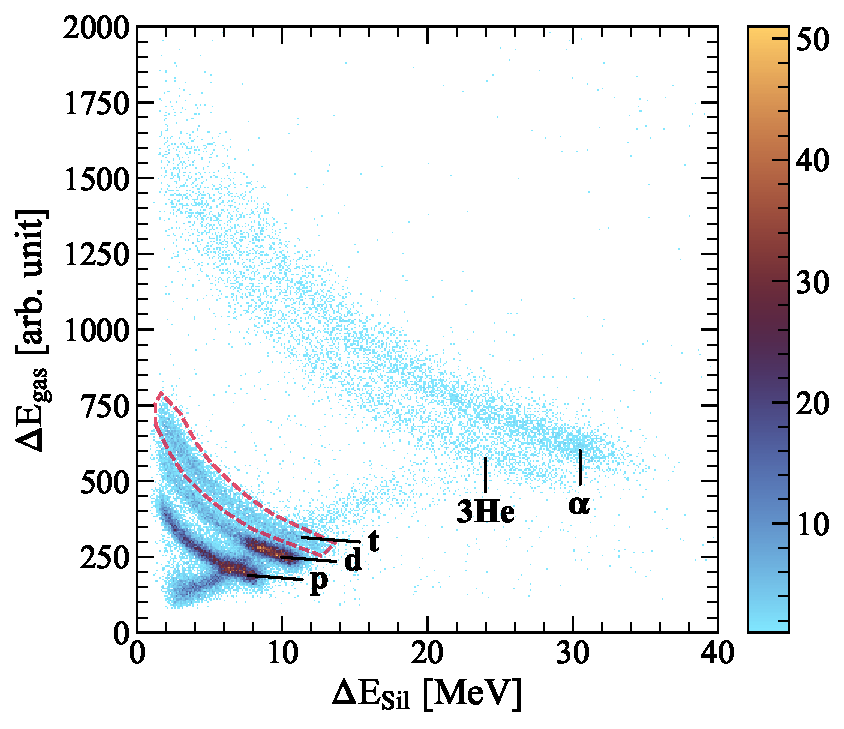
\includegraphics[width=0.95\linewidth]{figures/pid_front.pdf}
                \end{figure}
                \vspace*{-0.25cm}
                {\footnotesize\itshape Vetoing punch-through to 2nd front layer}
            }
        \end{column}%
        \begin{column}{0.5\linewidth}
            \mycolorbox[1]{box4}{
                \boxitem{2} Reconstruct $\text{E}_{\text{x}}$ by \textbf{missing-mass} technique
                \begin{figure}
                    \centering
                    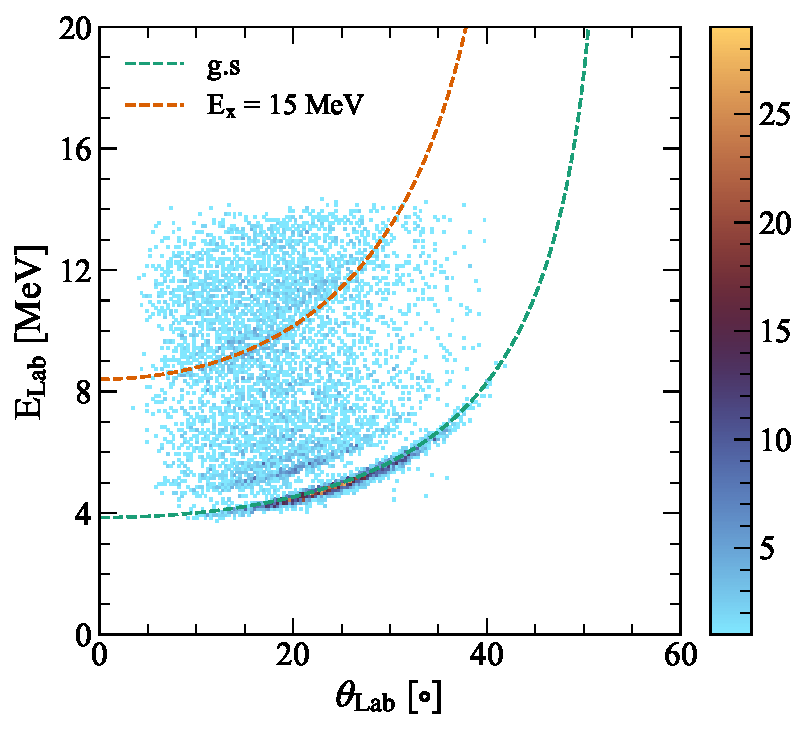
\includegraphics[width=0.95\linewidth]{figures/kin.pdf}
                \end{figure}
            }
        \end{column}
    \end{columns}

\end{frame}


\begin{frame}[plain]{Acknowledgments}
    \begin{columns}[T]
        \begin{column}{0.33\linewidth}
            % The E748 collaboration:
            \begin{itemize}\scriptsize
                \item Santiago:\\
                      B. Fernández\\
                      M. Caamaño\\
                      J. Lois
                \item LPC-Caen:\\
                      A. Matta\\
                      F. Delaunay\\
                      N. L. Achouri\\
                      F. Flavigny\\
                      J. Gibelin\\
                      M. Marques\\
                      N. Orr
                \item IJCLab:\\
                      D. Beaumel\\
                      M. Assié\\
                      Y. Blumenfeld\\
                      S. Franchoo\\
                      A. Georgiadou\\
                      V. Girard-Alcindor\\
                      F. Hammache\\
                      N. de Séreville\\
                      A. Meyer\\
                      I. Stefan
            \end{itemize}
        \end{column}
        \begin{column}{0.33\linewidth}
            \begin{itemize}\scriptsize
                \item GANIL:\\
                      B. Jacquot\\
                      O. Kamalou\\
                      A. Lemasson\\
                      M. Rejmund\\
                      T. Roger\\
                      O. Sorlin\\
                      J.C. Thomas\\
                      M. Vandebrouck\\
                      B. Bastin\\
                      F. de Oliveira\\
                      C. Stodel
                \item RIKEN:\\
                      S. Koyama\\
                      D. Suzuki
                \item Surrey:\\
                      N. Timofeyuk
            \end{itemize}

        \end{column}
        \begin{column}{0.33\linewidth}
            
\includegraphics[width=0.6\linewidth]{logos/usc_blue.png}\vspace{1em}
            
\includegraphics[width=0.6\linewidth]{logos/lpc.png}\vspace{1em}
            
\includegraphics[width=0.6\linewidth]{logos/ganil.png}\vspace{1em}
            
\includegraphics[width=0.6\linewidth]{logos/ijclab.png}\vspace{1em}
            
\includegraphics[width=0.6\linewidth]{logos/riken.png}\vspace{1em}
            
\includegraphics[width=0.6\linewidth]{logos/surrey.png}\vspace{1em}
        \end{column}
    \end{columns}
\end{frame}


\end{document}
